\newpage
\pdfbookmark[0]{\contentsname}{toc}
\tableofcontents*
\cleardoublepage
\newpage


\hrule	% Linha horizontal
\begin{center} % Minipage Centralizado
\begin{minipage}[c]{12.5cm} % Largura
Autor: \imprimirautor

Tema: \imprimirtitulo 
\imprimirlocal,\\ 
\imprimirorientador\\
\hspace{0.5cm}
\parbox[t]{\textwidth}{\imprimirinstituicao
\imprimirdata.}\\
\hspace{0.5cm}
\end{minipage}
\end{center}
\hrule

\vspace{1cm}

\SingleSpacing
\noindent
{\textbf{LEARNING ARTIFICIAL INTELLIGENCE THROUGH ARTIFICIAL MEMORIES}}
\indent
\small

Memories and attitudes contribute the conscious and the human character from diverse happenings, be they good or not. However, both contribute to learning. In the case of memories, the conscious directs the attitudes, demanding less brain processing. Artificial intelligence uses this same principle of events for its development, that is, the use of artificial memories theoretically could simulate human attitudes.

\noindent
 
\textbf{Keywords}: Intelligence,Artificial,Memories,Humans,Technology,Modern,World,
\\Consciousness,Through,Brain.

\SingleSpacing
\noindent
{\textbf{APRENDIZADO DE INTELIGÊNCIA ARTIFICIAL ATRAVÉS DE MEMÓRIAS ARTIFICIAIS}}
\indent
\small

Memórias e atitudes contribuem para a construção do consciente e o caráter humano a partir de diversos acontecimentos, sejam eles bons ou não, ambos contribuindo para o aprendizado. No caso das memórias, o consciente direciona as atitudes, demandando menos processamento do cérebro. A inteligência artificial usa desse mesmo princípio de acontecimentos para o seu desenvolvimento, ou seja, a utilização de memórias artificiais teoricamente poderiam simular atitudes humanas.

\noindent
 
\textbf{Palavras-Chave}: Inteligência,Artificial,Memórias,Humanas,Tecnologia,Moderno,Mundo,
\\Consciência,Através,Cérebro.

\vspace{2cm}

\section{Introdução}
“A inteligência artificial (IA), trouxe várias aplicações importantes para níveis de desempenho quase humanos” \cite{anthes}.
As pessoas mesmo involuntariamente possuem atos, estes que são aprendidos a partir de algum fato do seu cotidiano, ou por experiências passadas. Esses atos são armazenados em pequenas informações mnemônicas, o que pode direcionar na tomada de decisões \cite{buzsaki}. Estes autores afirmam que para a tomada de decisões ideais é necessário um mecanismo que integre as populações neurais distribuídas. Segundo \cite{eichenbaum}, essas decisões são tomadas a partir de memórias do hipocampo, que é uma estrutura que representa a memória para eventos passados.



\section{Revisão Sistemática}
Para confecção deste artigo, foi utilizada a técnica de Revisão Sistemática de Literatura(RSL). Esta possui o objetivo de realizar um trabalho de pesquisa e a partir deste trabalho, ser capaz de interpretar e analisar estudos sobre determinado assunto \cite{brereton}. Dyba, Kitchenham,  Jorgensen(2005), propuseram um processo que resume de forma sucinta como aplicar esta técnica.


\vspace{1cm}
\section{Planejamento da Pesquisa}
Este tópico aborda sobre a pesquisa realizada, pesquisa em bases de busca utilizadas na realização da pesquisa, além das palavras-chave e a \textit{String} de busca.

Com a intenção de encontrar uma maior variedade de artigos e revistas publicadas, foi escolhido o idioma inglês. Este idioma, por se tratar de um idioma conhecido no mundo inteiro e ser o principal idioma para publicações internacionais, o que auxiliou na procura de artigos relevantes para este trabalho.

Após ser definido o objetivo do trabalho e as questões de pesquisa que foram levantadas a partir deste, foram escolhidas palavras-chave que ajudasse na construção de strings de busca. Após estes tópicos serem contemplados, foi escolhido o idioma que abrange um público internacional maior, que é o idioma inglês. A letra “P” foi utilizada para abreviação da palavra “Palavra”.

Palavras-chave identificadas:

\begin{itemize}
	\item P01. \textit{Intelligence}
	\item P02. \textit{Artificial}
	\item P03. \textit{Memories}
	\item P04. \textit{Humans}
    \item P05. \textit{Technology}
    \item P06. \textit{Modern}
    \item P07. \textit{World}
    \item P08. \textit{Human}
    \item P09. \textit{Consciousness}
    \item P10. \textit{Brain}
\end{itemize}

Utilizando os tópicos anteriores de objetivos, questões de pesquisa, idioma escolhido e as palavras-chave, estas últimas serão utilizadas na próxima fase do processo da Figura 1. Estas palavras serão utilizadas como base para a especificação da \textit{String} de busca. As siglas “SB” a seguir, se referem as palavras “\textit{String} de busca”.

\begin{itemize}
    \item SB01: \textit{Intelligence artificial and modern world};
	\item SB02: \textit{Human Consciousness and Intelligence Artificial};
	\item SB03: \textit{Artificial Intelligence Through Memories};
    \item SB04: \textit{Artificial Learning and Intelligence Artificial}.
\end{itemize}

As bases de dados escolhidas para a elaboração deste trabalho, foram escolhidas pelas suas relevâncias de pesquisa e extensão. Utilizando a sigla de BD, que é um acrônimo para base de dados, as seguintes bases de dados foram usadas para aplicação da técnica de Revisão Sistemática de Literatura (RSL).

\begin{itemize}
    \item BD1. CAPES Periódicos;
    \item BD2. Google Academic.
\end{itemize} 

\subsection{Critérios de Inclusão}
\label{subsec:inclusao}

Após serem definidas as \textit{Strings} de busca e inseridas nas bases de dados, foram adotados alguns critérios para a escolha dos trabalhos já publicados. A sigla “CI” é a abreviação das palavras Critérios de Inclusão.

\begin{itemize}
    \item CI01. A publicação deve estar em inglês;
    \item CI02. A publicação deve estar disponível nas bases para download ou disponível para leitura online;
    \item CI03. A publicação deve necessariamente estar de acordo com o tema e os objetivos propostos.
\end{itemize}

\subsection{Critérios de Exclusão}
\label{subsec:exclusao}

Com a intenção de não ser aceito todos os artigos resultantes a partir da \textit{String} de busca, foram adotados alguns critérios para uma melhor escolha dos artigos aceitos. A sigla “CE” é a abreviação das palavras Critérios de Exclusão. 

\begin{itemize}
    \item CE01. A publicação não pode fugir do objetivo proposto.
\end{itemize}
\label{sec:planejamento}

\vspace{1cm}
\section{Execução da Revisão Sistemática}
Esta atividade é o ínicio da segunda fase do processo da Figura \ref{img:processo}, sendo a fase de execução. Nesta fase é a que utiliza toda a bagagem da primeira fase do processo e a executa, com o propósito de alcançar o objetivo deste trabalho.

\section{Execução da Busca}

Na execução desta atividade, foi utilizadas as \textit{Strings} de busca, definidas no tópico \ref{sec:planejamento}, e aplicadas nas bases de dados.

Com o intuito de selecionar os artigos que melhor se adeque ao tema, foram utilizados os critérios de inclusão. Os artigos resultantes da pesquisa utilizando a \textit{String} de busca e que atendiam aos critérios de inclusão, foram armazenados para uma posterior análise crítica deste trabalho.

Após feita a seleção das publicações, foram extraídos dados e informações que pudessem classificar as iniciativas e aumentar o entendimento do tópico em questão. As áreas mais recorrentes foram categorizadas em duas áreas: Inteligência artificial e Tomadas de Decisões. A escolha dessas duas categorias se deu ao fato de ser necessário entender primeiro como se a distribuição neural do cérebro humano e como essa distribuição pode auxiliar a inteligência artificial.

\begin{table}[h]
\centering
\begin{tabular}{ | l | l | p{5cm} | l | p{10cm} |}
\hline
\rowcolor[HTML]{F8FF00} 
{\color[HTML]{000000} \textbf{Categoria}} & \textbf{Ano} & \textbf{Título} & \textbf{Autores}        \\ \hline
{\cellcolor[HTML]{34FF34}}\textbf{Tomada de Decisão}               & 2013                   & Synchronization of Medial Temporal Lobe and Prefrontal Rhythms in Human Decision Making    & Guitart-Masip, Marc;Barnes          \\ \hline
 & 2007 & The medial temporal lobe and recognition memory & Eichenbaum H, Yonelinas AP\\ \hline
 & 2015 & Composite collective decision-making & Czaczkes, Tomer J ; Benjamin \\ \hline
 {\cellcolor[HTML]{34FF34}}\textbf{Inteligência Artificial} & 2017 & Artificial intelligence poised to ride a new wave & Anthes Gary \\ \hline
 & 2010 & Artificial Learning in Artificial Memories & Burger, John Robert \\ \hline
 & 2012 & Interdisciplinary Reviews: Computational Statistics & Tecuci, Gheorghe,Wiley \\ \hline
\end{tabular}
\caption{Categorização das Áreas de Pesquisa}
Fonte: Autor
\label{tab:categorizacao}
\end{table}

\vspace{1cm}
\section{Resultados da Revisão Sistemática}
As publicações foram analisadas e categorizadas, conforme mostra na Tabela \ref{tab:categorizacao}. As questões de pesquisa foram utilizadas para nortear um caminho a ser percorrido para alcançar o objetivo deste trabalho. A seguir será mostrada uma análise sobre categoria.

\section{Tomada de Decisões}

O cérebro humano possui diferentes formas de reconhecimento, duas delas podem ser exemplificadas como experiências subjetivas, tais como o senso de familiaridade e o senso da experiência. O primeiro é uma intuição fraca a uma crença convincentemente forte. O segundo é voltada a lembrança, o que envolve a recuperação de associações entre fatos, requisitando palavras ou ações para que o cérebro dê uma resposta.

Essas duas experiências no entendo, não podem ser ditos ao certo se os dois sensos são processados pelo cérebro de maneiras diferentes. De uma forma geral, a familiaridade é processada mais rapidamente em consideração a experiência. Por exemplo, quando uma pessoa passa por uma atividade que a ela já é comum, a requisição sobre o cérebro é menor do que comparado com a experiência, onde o cérebro necessita de um tempo maior para processar a situação sobre fatos que são ou não conhecidos por ele. 

A tomada de decisões é feita a partir de informações de memória armazenadas em regiões do cérebro, para tanto é necessário um mecanismo para a integração entre as informações neurais distribuídas \cite{buzsaki}. Este mecanismo provavelmente utilizará sinais do hipocampo,este que é considerada a principal sede de memória, para a representar a memória de eventos anteriores \cite{eichenbaum}.

A tomada de decisões pode ser feita a partir de habilidades cognitivas, como a memória, que lhes permitem aprimorar suas decisões. Segundo o filósofo \cite{aristoteles}, “O homem é um animal social por natureza”. Seguindo o pensamento do filósofo, os animais tomam decisões são adaptáveis conforme o grupo em que se encontra. Ao observar esse contexto, é esperado que atitudes tenham decisões diferentes de acordo com a situação. Esse processo de adaptação se baseia de acordo com experiências anteriores, sejam elas senso familiares ou senso de experiência.

Este modelo foi proposto como resultado de pesquisas sobre como o cérebro utiliza de diferentes tipos de experiência para uma tomada de decisão. Essa atitude pode ser tomada a partir de um fator como familiar ou por experiências cotidianas. A velocidade de processamento das informações depende do quão a atividade é exercida pela pessoa, o que leva o cérebro a tratar-las de modo mais rápido ou não. Como a tomada de decisão é exercida a partir de informações armazenadas no cérebro, os neurocientistas possuem um papel muito importante para auxiliar os pesquisadores de tecnologias que visam aprimorar ações de seres que podem ser construídos, como robôs.

\section{Inteligência Artificial}

Segundo \cite{anthes}, a Inteligência Artificial (IA) é uma tecnologia com potencial permanente. Como advento de suas descobertas, IA trouxe benefícios como reconhecimento de fala, automação da navegação de veículos, para níveis quase humanos.

Ainda segundo \cite{anthes}, especialistas na área de Inteligência Artificial afirmam que essa tecnologia pode permitir que sistemas sejam inteligentes ao ponto de entender e reagir ao mundo de um ponto de visto humano. 

\cite{john}, afirma que a aprendizagem pode ser vista no sentido biológico como um processo de internalização que detecta, lembra e reproduz sequências bem sucedidas. Resultados de aprendizado ao executar uma ação ou possivelmente várias ações ao mesmo tempo sem esforço cognitivo ou pensamento, ou seja, sem envolvimento consciente.

O hardware de memória é projetado para aprender ações repetidas, sendo feita uma analogia ao aprendizado humano. Ações comuns são mapeadas na memória e podem ser executadas sem esforço da CPU (análogo ao pensamento). Propriedades de IA para sequências mapeadas na memória estão na tabela \ref{tab:artificial}.

\begin{table}[H]
\centering
\begin{tabular}{|c|c|}
\hline
1 & A result of rehearsal                    \\ \hline
2 & Occurs within long term memory \\ \hline
3 & Enables long term modification of underlying circuitry \\ \hline
4 & Permits action without CPU effort \\ \hline
5 & Permits action without CPU delays \\ \hline
6 & Permits action without CPU memory usage \\ \hline
7 & Independent sequences may run concurrently \\ \hline
\end{tabular}
\caption{Artificial Learning}
Fonte: \cite{john}
\label{tab:artificial}
\end{table}

Para melhor enfatizar a tabela \ref{tab:artificial}, ela será traduzida para a língua portuguesa brasileira a seguir:

\begin{table}[H]
\centering
\begin{tabular}{|c|c|}
\hline
1 & Um resultado do ensaio                    \\ \hline
2 & Ocorre dentro da memória de longo prazo \\ \hline
3 & Permite a modificação a longo prazo dos circuitos subjacentes \\ \hline
4 & Permite ação sem esforço da CPU \\ \hline
5 & Permite ação sem atrasos de CPU \\ \hline
6 & Permite ação sem uso de memória da CPU \\ \hline
7 & Sequências independentes podem ser executadas simultaneamente \\ \hline
\end{tabular}
\caption{Aprendizado Artificial}
Fonte: \cite{john} com Adaptações
\label{tab:artificialtraduzido}
\end{table}

\begin{figure}[H]
		\centering
		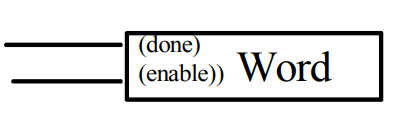
\includegraphics[width=14.5cm]{figuras/sinaisdememoria}
        \caption{Símbolo para uma palavra de memória de longo prazo com controles}
        Fonte: \cite{john}
		\label{img:palavra}
\end{figure}

Para entender a Figura \ref{img:palavra}, deve se entender primeiro o que é uma memória a longo prazo. Esta memória é a capacidade de se manter uma informação recente de poucos dias ou até décadas. Se difere da memória a curto prazo, pois esta pode armazenar elementos por uns 20-30 segundos.

Nesse contexto, a memória a longo prazo pode ser uma ou um conjunto de palavras, que emitem sinais e comandos quando acionadas, ativando o \textit{enable}, como visto na Figura \ref{img:palavra}. Para o aprendizado de algo que está sendo praticado, é necessário um filtro de tempo para detectar uma repetição ou sequência \cite{john}. Para exemplificar este comportamento, imagine um filtro que detecte sempre que uma determinada palavra é ativada após outra palavra dada é feita. A repetição ou sequência dessa palavra seguida de uma ordem é apreendida pela memória e assim armazenada.

Nesse viés, a IA utiliza dados como entrada e esses dados repetidos, por exemplo palavras, são armazenadas como memórias a longo prazo. Essas memórias, usa do princípio inicial da Inteligência Artificial de aprender conforme a inserção dos dados e responder conforme esses dados. Seguindo essa lógica, tem-se o advento do aprendizado de máquina recorrente de dados externos, no caso da IA, e conforme a inserção de mais dados, maiores e mais diferentes serão as atitudes que serão realizadas por ela.

\vspace{1cm}
\section{Considerações Finais}
Este trabalho buscou averiguar se é possível a simulação de atividades humanas por meio da tecnologia de Inteligência Artificial. A conscientização de tecnologias que tentam aproximar decisões humanas a máquinas já são empregadas em nosso cotidiano, como carros com navegação personalizada, sistemas embutidos de inteligência artificial em \textit{smartphones}, como no caso da \textit{SIRI} e \textit{Android} para as empresas internacionais \text{Apple} e \textit{Google} respectivamente.

Para a confecção deste trabalho foi aplicada a técnica de Revisão Sistemática de Literatura (RSL) para direcionar um método de pesquisa e assim organizar as publicações conforme o tema, em bases de dados selecionadas, sendo feita a partir de palavras-chave e \textit{string} de busca.

As publicações foram escolhidas a partir dos critérios de inclusão e o conjunto de publicações que não foram selecionadas, foram excluídas a partir do critério de exclusão. As publicações foram categorizadas em duas categorias: Tomada de Decisões e Inteligência Artificial. A maior parte dos artigos selecionados, foram publicados nos últimos 20 anos. Com a realização da pesquisa deste trabalho, foi possível alcançar resultados favoráveis aos objetivos desejados. Foi constatado que existem estudos na área com potenciais para o desenvolvimento de sistemas artificiais que interajam de forma mais humana. Esses sistemas poderão simular sentimentos e ações humanas, e se adaptar conforme o conjunto social em que esteja envolvido.

Após a análise dos dados deste trabalho, é verificado que existe a possibilidade de desenvolvimento para novos trabalhos, envolvendo o desenvolvimento da Inteligência Artificial e tecnologias emergentes. Para um melhor desenvolvimento dessa área, pesquisadores de IA poderiam estudar mais como funciona o cérebro humano e a partir disso aplicar esses estudos na tecnologia, o que poderia levar a resultados mais próximos do desejado.